\documentclass{ximera}

\graphicspath{  
{./}
{./whoAreYou/}
{./drawingWithTheTurtle/}
{./bisectionMethod/}
{./circles/}
{./anglesAndRightTriangles/}
{./lawOfSines/}
{./lawOfCosines/}
{./plotter/}
{./staircases/}
{./pitch/}
{./qualityControl/}
{./symmetry/}
{./nGonBlock/}
}


%% page layout
\usepackage[cm,headings]{fullpage}
\raggedright
\setlength\headheight{13.6pt}


%% fonts
\usepackage{euler}

\usepackage{FiraMono}
\renewcommand\familydefault{\ttdefault} 
\usepackage[defaultmathsizes]{mathastext}
\usepackage[htt]{hyphenat}

\usepackage[T1]{fontenc}
\usepackage[scaled=1]{FiraSans}

%\usepackage{wedn}
\usepackage{pbsi} %% Answer font


\usepackage{cancel} %% strike through in pitch/pitch.tex


%% \usepackage{ulem} %% 
%% \renewcommand{\ULthickness}{2pt}% changes underline thickness

\tikzset{>=stealth}

\usepackage{adjustbox}

\setcounter{titlenumber}{-1}

%% journal style
\makeatletter
\newcommand\journalstyle{%
  \def\activitystyle{activity-chapter}
  \def\maketitle{%
    \addtocounter{titlenumber}{1}%
                {\flushleft\small\sffamily\bfseries\@pretitle\par\vspace{-1.5em}}%
                {\flushleft\LARGE\sffamily\bfseries\thetitlenumber\hspace{1em}\@title \par }%
                {\vskip .6em\noindent\textit\theabstract\setcounter{question}{0}\setcounter{sectiontitlenumber}{0}}%
                    \par\vspace{2em}
                    \phantomsection\addcontentsline{toc}{section}{\thetitlenumber\hspace{1em}\textbf{\@title}}%
                     }}
\makeatother



%% thm like environments
\let\question\relax
\let\endquestion\relax

\newtheoremstyle{QuestionStyle}{\topsep}{\topsep}%%% space between body and thm
		{}                      %%% Thm body font
		{}                              %%% Indent amount (empty = no indent)
		{\bfseries}            %%% Thm head font
		{)}                              %%% Punctuation after thm head
		{ }                           %%% Space after thm head
		{\thmnumber{#2}\thmnote{ \bfseries(#3)}}%%% Thm head spec
\theoremstyle{QuestionStyle}
\newtheorem{question}{}



\let\freeResponse\relax
\let\endfreeResponse\relax

%% \newtheoremstyle{ResponseStyle}{\topsep}{\topsep}%%% space between body and thm
%% 		{\wedn\bfseries}                      %%% Thm body font
%% 		{}                              %%% Indent amount (empty = no indent)
%% 		{\wedn\bfseries}            %%% Thm head font
%% 		{}                              %%% Punctuation after thm head
%% 		{3ex}                           %%% Space after thm head
%% 		{\underline{\underline{\thmname{#1}}}}%%% Thm head spec
%% \theoremstyle{ResponseStyle}

\usepackage[tikz]{mdframed}
\mdfdefinestyle{ResponseStyle}{leftmargin=1cm,linecolor=black,roundcorner=5pt,
, font=\bsifamily,}%font=\wedn\bfseries\upshape,}


\ifhandout
\NewEnviron{freeResponse}{}
\else
%\newtheorem{freeResponse}{Response:}
\newenvironment{freeResponse}{\begin{mdframed}[style=ResponseStyle]}{\end{mdframed}}
\fi



%% attempting to automate outcomes.

%% \newwrite\outcomefile
%%   \immediate\openout\outcomefile=\jobname.oc
%% \renewcommand{\outcome}[1]{\edef\theoutcomes{\theoutcomes #1~}%
%% \immediate\write\outcomefile{\unexpanded{\outcome}{#1}}}

%% \newcommand{\outcomelist}{\begin{itemize}\theoutcomes\end{itemize}}

%% \NewEnviron{listOutcomes}{\small\sffamily
%% After answering the following questions, students should be able to:
%% \begin{itemize}
%% \BODY
%% \end{itemize}
%% }
\usepackage[tikz]{mdframed}
\mdfdefinestyle{OutcomeStyle}{leftmargin=2cm,rightmargin=2cm,linecolor=black,roundcorner=5pt,
, font=\small\sffamily,}%font=\wedn\bfseries\upshape,}
\newenvironment{listOutcomes}{\begin{mdframed}[style=OutcomeStyle]After answering the following questions, students should be able to:\begin{itemize}}{\end{itemize}\end{mdframed}}



%% my commands

\newcommand{\snap}{{\bfseries\itshape\textsf{Snap!}}}
\newcommand{\flavor}{\link[\snap]{https://snap.berkeley.edu/}}
\newcommand{\mooculus}{\textsf{\textbf{MOOC}\textnormal{\textsf{ULUS}}}}


\usepackage{tkz-euclide}
\tikzstyle geometryDiagrams=[rounded corners=.5pt,ultra thick,color=black]
\colorlet{penColor}{black} % Color of a curve in a plot



\ifhandout\newcommand{\mynewpage}{\newpage}\else\newcommand{\mynewpage}{}\fi


\author{Jenny Sheldon \and Bart Snapp}


\outcome{}


\title{Symmetry groups}

\begin{document}
\begin{abstract}
  We look at all the symmetries of an object.
\end{abstract}
\maketitle


Now let's mix our rotations and reflections.  Consider our original
triangle and apply $\mat{F}_\ell \mat{R}_{120}$:
\begin{image}
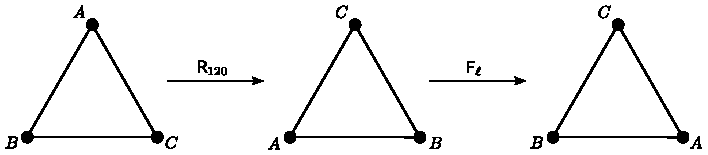
\includegraphics{symTriComp1.pdf}
\end{image}
What you may not immediately notice is that we obtain the same
transformation by taking the original triangle and applying
$\mat{F}_m$.
\begin{image}
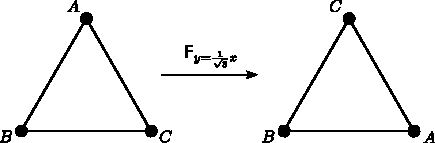
\includegraphics{symTriComp2.pdf}
\end{image}



As it turns out, every possible symmetry of the equilateral triangle
can be represented using reflections and rotations.  Each of these
reflections and rotations can be expressed as a composition of a
single reflection and a single rotation.  The collection of all
symmetries forms a group called the \index{symmetry
  group}\textit{symmetry group} of the equilateral triangle. 
\begin{image}
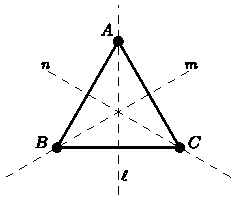
\includegraphics{symTriRef.pdf}
\end{image}
Let's see the group table.  Remember that we let $\mat{R} = \mat{R}_{120}$
and $\mat{F} = \mat{F}_{\l}$:

\[
{
\renewcommand{\arraystretch}{1.2}
\begin{array}{| c || c | c | c |c | c | c |}
\hline
\circ & \mat{I} & \mat{R} & \mat{R}^2  & \mat{F} & \mat{F} \mat{R} &  \mat{F} \mat{R}^2  \\ \hline \hline
\mat{I} & \mat{I} & \mat{R} & \mat{R}^2 & \mat{F} & \mat{F} \mat{R} & \mat{F} \mat{R}^2 \\ \hline
\mat{R} & \mat{R} & \mat{R}^2 & \mat{I} & \mat{F} \mat{R}^2 & \mat{F} & \mat{F} \mat{R} \\ \hline
\mat{R}^2 & \mat{R}^2 & \mat{I} & \mat{R} & \mat{F} \mat{R} & \mat{F} \mat{R}^2 & \mat{F}  \\ \hline
\mat{F} & \mat{F} & \mat{F} \mat{R} & \mat{F} \mat{R}^2 & \mat{I} & \mat{R} & \mat{R}^2 \\ \hline
\mat{F} \mat{R} & \mat{F} \mat{R} & \mat{F} \mat{R}^2 & \mat{F} & \mat{R}^2 & \mat{I} & \mat{R}  \\ \hline
\mat{F} \mat{R}^2 & \mat{F} \mat{R}^2 & \mat{F} & \mat{F} \mat{R} & \mat{R} & \mat{R}^2 & \mat{I}\\ \hline
\end{array}}
\]

This table shows every symmetry of the triangle, including the
identity $\mat{I}$. By comparing the rows and columns of the group
table, you can see that every element has an inverse. Combined
with the fact that the matrix multiplication is associative, this shows that
the symmetries of the triangle,
\[
\{ \mat{I},\mat{R},\mat{R}^2,\mat{F},\mat{F} \mat{R},  \mat{F} \mat{R}^2\}
\]
form a group.

\begin{question} 
Can you express the symmetries of the square in terms of reflections
and rotations? What does the group table look like for the symmetry
group of the square?
\end{question}



\end{document}
